\documentclass{beamer}
\mode<presentation>{
  \usetheme{Boadilla}
  \usefonttheme[onlylarge]{structurebold}
  \usefonttheme[stillsansseriflarge]{serif}
  \setbeamerfont*{frametitle}{size=\normalsize,series=\bfseries}
  % \setbeamertemplate{navigation symbols}{}
  \setbeamercovered{transparent}
}
\usepackage[english]{babel}
\usepackage[latin1]{inputenc}
\usepackage{times}
\usepackage[T1]{fontenc}
\usepackage{amsmath}
\usepackage{amssymb}
\usepackage{esint}
\usepackage{hyperref}
\usepackage{tikz}
\usepackage{xkeyval}
\usepackage{xargs}
\usepackage{verbatim}
\usetikzlibrary{
  arrows,
  calc,
  decorations.pathmorphing,
  decorations.pathreplacing,
  decorations.markings,
  fadings,
  positioning,
  shapes
}

\mode<handout>{
  \usepackage{pgfpages}
  \pgfpagesuselayout{4 on 1}[a4paper,landscape,border shrink=5mm]
  \setbeamercolor{background canvas}{bg=black!10}
}

\newcommand\pgfmathsinandcos[3]{%
  \pgfmathsetmacro#1{sin(#3)}%
  \pgfmathsetmacro#2{cos(#3)}%
}
\newcommand\LongitudePlane[3][current plane]{%
  \pgfmathsinandcos\sinEl\cosEl{#2} % elevation
  \pgfmathsinandcos\sint\cost{#3} % azimuth
  \tikzset{#1/.estyle={cm={\cost,\sint*\sinEl,0,\cosEl,(0,0)}}}
}
\newcommand\LatitudePlane[3][current plane]{%
  \pgfmathsinandcos\sinEl\cosEl{#2} % elevation
  \pgfmathsinandcos\sint\cost{#3} % latitude
  \pgfmathsetmacro\yshift{\cosEl*\sint}
  \tikzset{#1/.estyle={cm={\cost,0,0,\cost*\sinEl,(0,\yshift)}}} %
}
\newcommand\DrawLongitudeCircle[2][1]{
  \LongitudePlane{\angEl}{#2}
  \tikzset{current plane/.prefix style={scale=#1}}
  % angle of "visibility"
  \pgfmathsetmacro\angVis{atan(sin(#2)*cos(\angEl)/sin(\angEl))} %
  \draw[current plane] (\angVis:1) arc (\angVis:\angVis+180:1);
  \draw[current plane,dashed] (\angVis-180:1) arc (\angVis-180:\angVis:1);
}
\newcommand\DrawLatitudeCircleArrow[2][1]{
  \LatitudePlane{\angEl}{#2}
  \tikzset{current plane/.prefix style={scale=#1}}
  \pgfmathsetmacro\sinVis{sin(#2)/cos(#2)*sin(\angEl)/cos(\angEl)}
  % angle of "visibility"
  \pgfmathsetmacro\angVis{asin(min(1,max(\sinVis,-1)))}
  \draw[current plane,decoration={markings, mark=at position 0.6 with {\arrow{<}}},postaction={decorate},line width=.6mm] (\angVis:1) arc (\angVis:-\angVis-180:1);
  \draw[current plane,dashed,line width=.6mm] (180-\angVis:1) arc (180-\angVis:\angVis:1);
}
\newcommand\DrawLatitudeCircle[2][1]{
  \LatitudePlane{\angEl}{#2}
  \tikzset{current plane/.prefix style={scale=#1}}
  \pgfmathsetmacro\sinVis{sin(#2)/cos(#2)*sin(\angEl)/cos(\angEl)}
  % angle of "visibility"
  \pgfmathsetmacro\angVis{asin(min(1,max(\sinVis,-1)))}
  \draw[current plane] (\angVis:1) arc (\angVis:-\angVis-180:1);
  \draw[current plane,dashed] (180-\angVis:1) arc (180-\angVis:\angVis:1);
}
\newcommand\coil[1]{
  {\rh * cos(\t * pi r)}, {\apart * (2 * #1 + \t) + \rv * sin(\t * pi r)}
}
\makeatletter
\define@key{DrawFromCenter}{style}[{->}]{
  \tikzset{DrawFromCenterPlane/.style={#1}}
}
\define@key{DrawFromCenter}{r}[1]{
  \def\@R{#1}
}
\define@key{DrawFromCenter}{center}[(0, 0)]{
  \def\@Center{#1}
}
\define@key{DrawFromCenter}{theta}[0]{
  \def\@Theta{#1}
}
\define@key{DrawFromCenter}{phi}[0]{
  \def\@Phi{#1}
}
\presetkeys{DrawFromCenter}{style, r, center, theta, phi}{}
\newcommand*\DrawFromCenter[1][]{
  \setkeys{DrawFromCenter}{#1}{
    \pgfmathsinandcos\sint\cost{\@Theta}
    \pgfmathsinandcos\sinp\cosp{\@Phi}
    \pgfmathsinandcos\sinA\cosA{\angEl}
    \pgfmathsetmacro\DX{\@R*\cost*\cosp}
    \pgfmathsetmacro\DY{\@R*(\cost*\sinp*\sinA+\sint*\cosA)}
    \draw[DrawFromCenterPlane] \@Center -- ++(\DX, \DY);
  }
}
\newcommand*\DrawFromCenterText[2][]{
  \setkeys{DrawFromCenter}{#1}{
    \pgfmathsinandcos\sint\cost{\@Theta}
    \pgfmathsinandcos\sinp\cosp{\@Phi}
    \pgfmathsinandcos\sinA\cosA{\angEl}
    \pgfmathsetmacro\DX{\@R*\cost*\cosp}
    \pgfmathsetmacro\DY{\@R*(\cost*\sinp*\sinA+\sint*\cosA)}
    \draw[DrawFromCenterPlane] \@Center -- ++(\DX, \DY) node {#2};
  }
}
\makeatother

% not mandatory, but I though it was better to set it blank
\setbeamertemplate{headline}{}
\def\beamer@entrycode{\vspace{-\headheight}}

\tikzstyle{snakearrow} = [decorate, decoration={pre length=0.2cm,
  post length=0.2cm, snake, amplitude=.4mm,
  segment length=2mm},thick, ->]

%% document-wide tikz options and styles

\tikzset{%
  >=latex, % option for nice arrows
  inner sep=0pt,%
  outer sep=2pt,%
  mark coordinate/.style={inner sep=0pt,outer sep=0pt,minimum size=3pt,
    fill=black,circle}%
}
\def\timeleft{15:00->14:55}

\title[M�ssbauer Spectroscopy\hspace{2em}\tiny{\timeleft}]{M�ssbauer Spectroscopy}
\author{Yichao Yu}
\institute{MIT}

\begin{document}

\begin{frame}{}
  \titlepage
\end{frame}

\def\timeleft{14:55->14:20}
\begin{frame}{}
  \begin{block}{M�ssbauer effect and M�ssbauer spectroscopy.}
    \begin{itemize}[<+->]
    \item
      Nuclear $\gamma$ spectrum.
    \item
      Simple setup.
    \item
      Super high resolution. $(10^{12})$
    \end{itemize}
  \end{block}
  \begin{center}
    \includegraphics[width=7cm]{../all_data/02-28-FeC2O4_raw.png}\\
    M�ssbauer spectrum of $FeC_2O_4$.
  \end{center}
\end{frame}

\def\timeleft{14:20->13:50}
\begin{frame}
  \tableofcontents
\end{frame}

\def\timeleft{13:50->11:40}
\section{M�ssbauer effect.}
\begin{frame}{Nuclear spectrum and recoil.}
  \begin{columns}
    \column{6cm}
    \begin{block}{}
      \begin{itemize}[<+->]
      \item
        Radio active element radiate $\gamma$-ray at characteristic frequencies.
      \item
        Radiation $\rightarrow$ Absorption.
      \item
        Recoil momentum and doppler shift.
      \end{itemize}
    \end{block}
    \column{6cm}
    \only<1-2>{
      \visible<2>{
        \begin{center}
          \vspace{.95cm}
          \begin{tikzpicture}[scale=.8]
            \draw[line width=2] (0, 0) -- (2, 0);
            \draw[line width=2] (0, 3) -- (2, 3);
            \draw[->, line width=2] (1, 3) -- (1, 0);
            \draw[->, decorate, decoration=snake, line width=1] (1.5, 1.5) -- (4.5, 1.5);
            \path (3, 1.5) node[below] {$h\nu$};
            \draw[line width=2] (4, 0) -- (6, 0);
            \draw[line width=2] (4, 3) -- (6, 3);
            \draw[->, line width=2] (5, 0) -- (5, 3);
          \end{tikzpicture}\\\vspace{1cm}
        \end{center}
      }
    }
    \only<3>{
      \begin{center}
        \begin{tikzpicture}[scale=.8]
          \draw plot[id=x,domain=0:5,samples=1000] function{2 / (1 + 2 * (x - 2.3)**2)};
          \draw plot[id=x,domain=0:5,samples=1000] function{2 / (1 + 2 * (x - 2.7)**2)};
          \draw[->, black] (0, 0) -- (5, 0);
          \draw[->, black, line width=1] (2.3, 2) -- (2.7, 2);
          \draw[dashed] (2.3, 0) -- (2.3, 2);
          \draw[dashed] (2.7, 0) -- (2.7, 2);
          \path (2.5, 0) node[below] {Atom};
        \end{tikzpicture}\\\vspace{.5cm}
        \begin{tikzpicture}[scale=.8]
          \draw plot[id=x,domain=0:5,samples=1000] function{2 / (1 + 25 * (x - 2.1)**2)};
          \draw plot[id=x,domain=0:5,samples=1000] function{2 / (1 + 25 * (x - 2.9)**2)};
          \draw[->, black] (0, 0) -- (5, 0);
          \draw[->, black, line width=1] (2.1, 2) -- (2.9, 2);
          \draw[dashed] (2.1, 0) -- (2.1, 2);
          \draw[dashed] (2.9, 0) -- (2.9, 2);
          \path (2.5, 0) node[below] {Nuclear};
        \end{tikzpicture}
      \end{center}
    }
  \end{columns}
\end{frame}

\def\timeleft{11:40->10:00}
\begin{frame}{M�ssbauer effect.}
  \begin{columns}
    \column{6cm}
    \begin{block}{}
      \begin{itemize}[<+->]
      \item
        Discoveried in $1957$ by M�ssbauer.
      \item
        Momentum transfer with the whole cristal. $\rightarrow$ Recoilless.
      \item
        Scanning frequency using doppler effect.
      \end{itemize}
    \end{block}
    \column{6cm}
    \only<3>{
      \begin{tikzpicture}[scale=.8]
        \path (0, 0) node[below] {Target};
        \path (3, 0) node[below] {Source};
        \draw[line width=1] (0, 0) -- (0, 2);
        \draw[line width=1] (3, 0) -- (3, 2);
        \draw[<->, black, line width=1] (1, 2.2) -- (5, 2.2);
      \end{tikzpicture}
    }
  \end{columns}
\end{frame}

\def\timeleft{10:00 -> 7:30}
\section{Apparatus and samples.}
\begin{frame}{Experiment Apparatus.}
  \begin{tikzpicture}[scale=.8]
    \path (2, 0) node[below] {Source};
    \draw[line width=.5] (3.5, .9) -- (2.2, .9);
    \draw[line width=.5] (2.2, 1.1) -- (3.5, 1.1);
    \draw[line width=1] (3.5, 0) -- (3.5, 2);
    \draw[line width=1] (2.2, 0.8) -- (2.2, 1.2) -- (1.8, 1.2) -- (1.8, 0.8) -- cycle;
    \draw[<->, dashed, black, line width=1] (.6, 2.2) -- (3.4, 2.2);
    \uncover<4-> {
      \draw[line width=.5] (3.5, .9) -- (4.2, .9);
      \draw[line width=.5] (4.2, 1.1) -- (3.5, 1.1);

      \draw[line width=1] (4.4, 1.5) -- (4.4, 0.5);
      \draw[line width=.2] (4.4, 1.5) -- ++(-.2, -.2);
      \draw[line width=.2] (4.4, 1.3) -- ++(-.2, -.2);
      \draw[line width=.2] (4.4, 1.1) -- ++(-.2, -.2);
      \draw[line width=.2] (4.4, 0.9) -- ++(-.2, -.2);
      \draw[line width=.2] (4.4, 0.7) -- ++(-.2, -.2);

      \draw[line width=.5] (5.5, 0.5) -- (6.5, 1.5);

      \draw[line width=1] (5.5, -.3) -- (6.5, -.3);
      \draw[line width=.2] (5.5, -.3) -- ++(.2, -.2);
      \draw[line width=.2] (5.7, -.3) -- ++(.2, -.2);
      \draw[line width=.2] (5.9, -.3) -- ++(.2, -.2);
      \draw[line width=.2] (6.1, -.3) -- ++(.2, -.2);
      \draw[line width=.2] (6.3, -.3) -- ++(.2, -.2);

      \draw[line width=1] (7.5, 1.2) -- (7.5, 0.8) -- (8.5, 0.8) -- (8.5, 1.2) -- cycle;
      \path (8, 0.8) node[below] {Laser};

      \draw[line width=1] (5.8, 2.3) -- (6.2, 2.3) arc (0:180:.2);
      \path (6, 2.5) node[above] {Photo Diode};

      \draw[line width=1, red] (4.4, 1) -- (7.5, 1);
      \draw[line width=1, red] (6, 2.3) -- (6, -.3);
    }

    \uncover<2-> {
      \path (-2, 0) node[below] {Detector};
      \draw[line width=1] (-2.2, 0) -- (-2.2, 2) -- (-1.8, 2) -- (-1.8, 0) -- cycle;
    }

    \uncover<3-> {
      \path (0, 0) node[below] {Target};
      \draw[line width=1] (0, 0) -- (0, 2);
    }
  \end{tikzpicture}
  \visible<4->{
    \begin{block}{}
      \begin{itemize}
      \item<4->Velocity of the source,
        \[v=2f\lambda\]
      \item<5->
        Source: ${}^{57}Co$.
      \item<6->
        First decay into excited state of ${}^{57}Fe$.
      \item<7->
        Energy $14.4keV$.
      \end{itemize}
    \end{block}
  }
\end{frame}

\def\timeleft{7:30 -> 4:00}
\begin{frame}{Effects and samples.}
  \begin{columns}
    \column{5.5cm}
    \begin{block}{Effects}
      \begin{itemize}[<+->]
      \item
        \alert<6, 7, 8>{Isomer Shift.}
      \item
        \alert<5, 8>{Zeeman effect.}
        \[E=-g_N\mu_NBm_I\]
      \item
        \alert<6, 8>{Quadrapole Splitting.}
      \item
        \alert<9>{Temperature Shift.}
        \[\frac{\delta}{E}=\frac{v^2}{2c^2}=\frac{E_k}{mc^2}\]
      \end{itemize}
    \end{block}
    \column{5.5cm}
    \only<1> {
      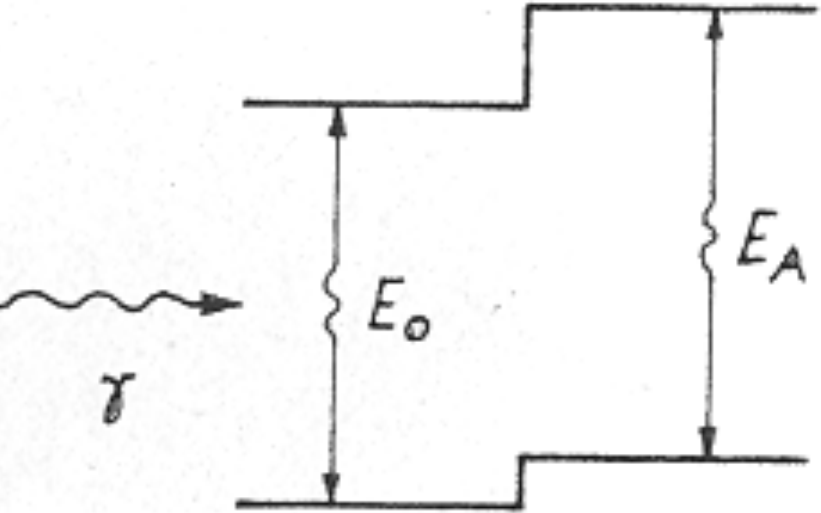
\includegraphics[width=6cm]{../share/isomer.png}
    }
    \only<2> {
      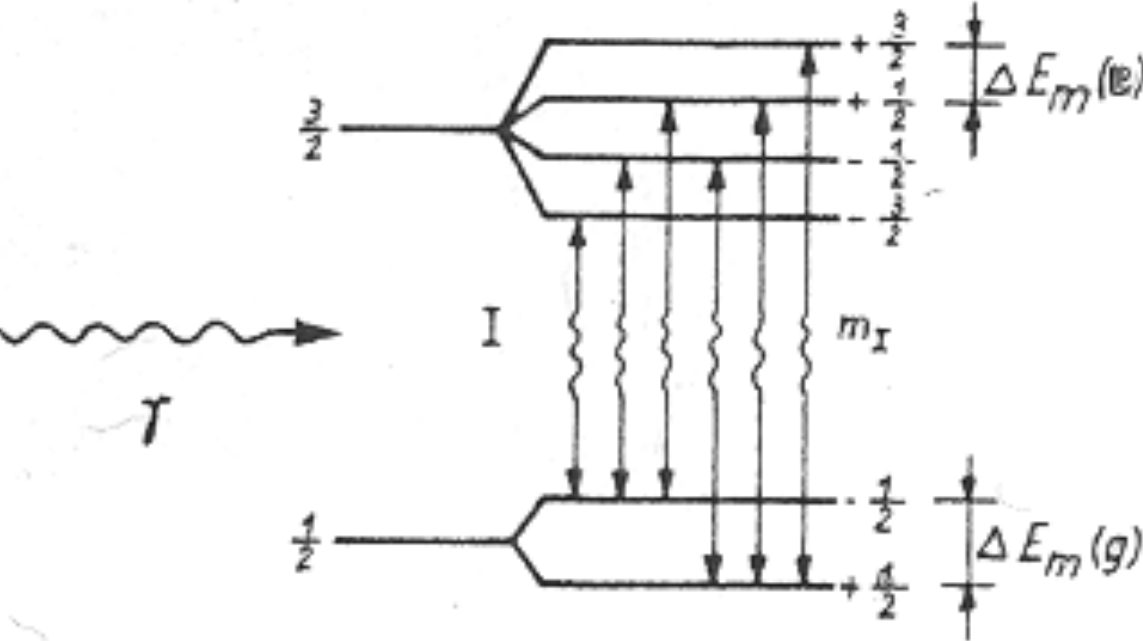
\includegraphics[width=6cm]{../share/zeeman.png}
    }
    \only<3> {
      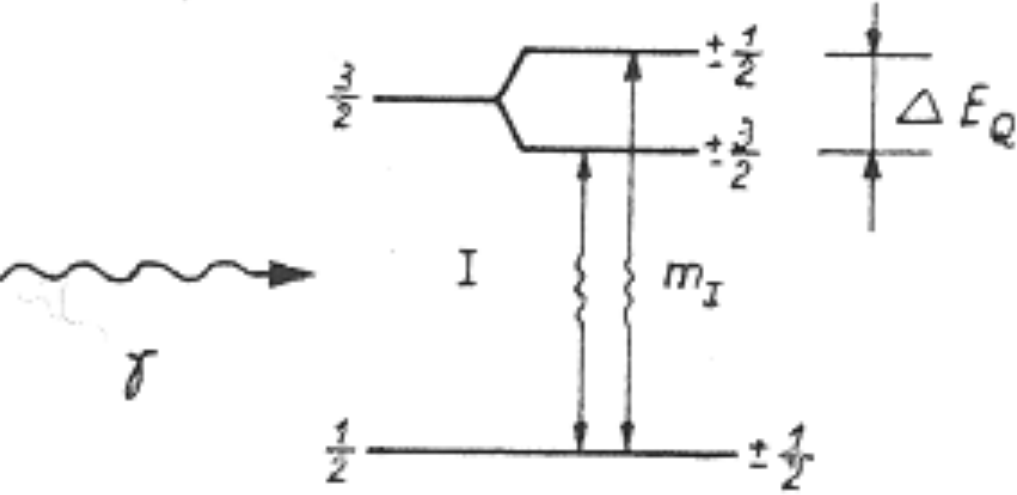
\includegraphics[width=6cm]{../share/quad.png}
    }
    \only<4> {
      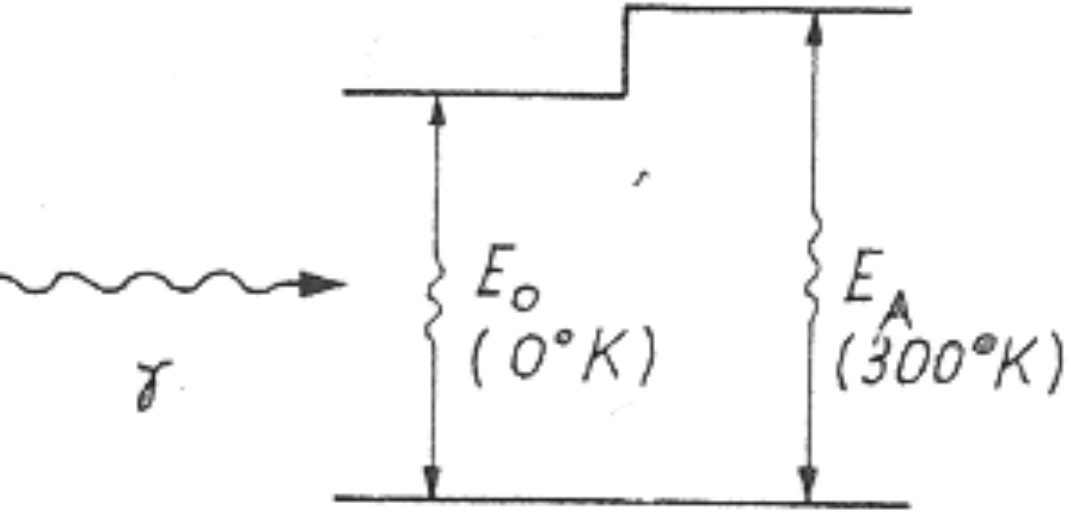
\includegraphics[width=6cm]{../share/temp.png}
    }
    \only<5-> {
      \begin{block}{Samples}
        \begin{itemize}[<+->]
        \item
          \alert<11>{${}^{57}Fe$}
        \item
          \alert<11>{$FeSO_4$}
        \item
          $Fe_2(SO_4)_3$
        \item
          $Fe_2O_3$
        \item
          \alert<11>{Stainless steel (Varying temperature).}
        \item
          $Na_4Fe(CN)_6$ For line width.
        \end{itemize}
      \end{block}
    }
  \end{columns}
\end{frame}

\def\timeleft{4:00->3:00}
\section{Data and result.}
\begin{frame}{Calibration.}
  \begin{columns}
    \column{6cm}
    \visible<+->{
      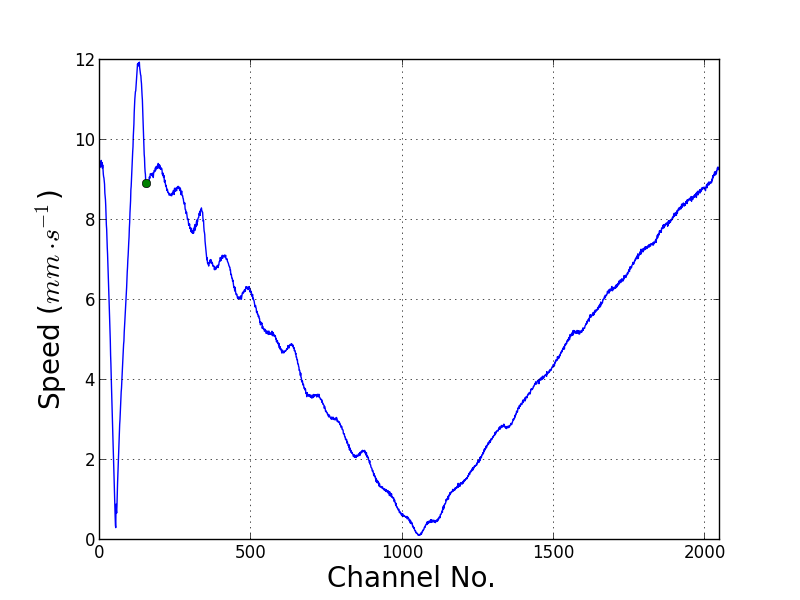
\includegraphics[width=6cm]{../pos_cal/res_v_raw.png}
    }
    \column{6cm}
    \visible<+->{
      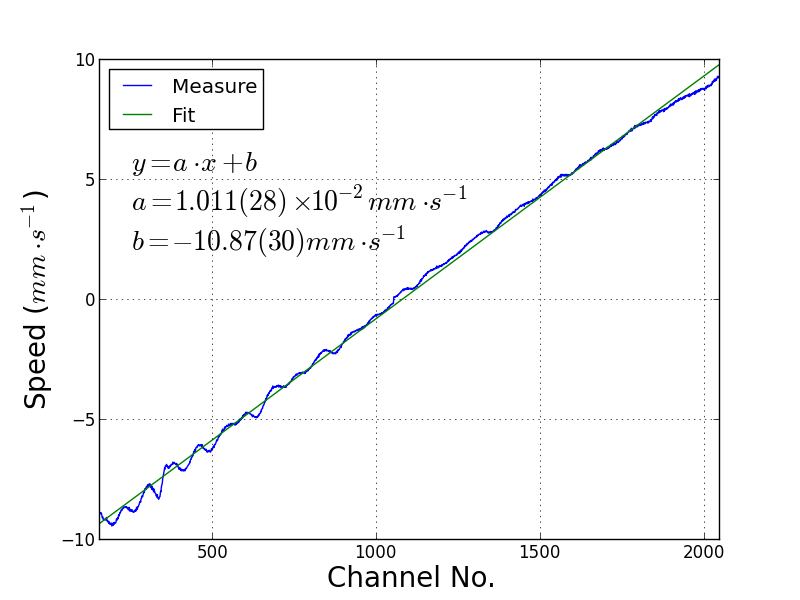
\includegraphics[width=6cm]{../pos_cal/res_v_fit.png}
    }
  \end{columns}
\end{frame}

\def\timeleft{3:00->2:00}
\begin{frame}{${}^{57}Fe$ and $FeSO_4$.}
  \begin{columns}
    \column{5.5cm}
    \visible<+->{
      \begin{center}
        ${}^{57}Fe$\\
        \includegraphics[width=6cm]{../pos_cal/02-14-6_2_raw.png}\\
        \begin{block}{Zeeman splitting for ground state ($g_0$) and excited state ($g_1$).}
          \begin{tabular}{|c|c|}
            \hline
            $g_0$&$1.882(13)\cdot10^{-7}eV$\\\hline
            $g_1$&$1.074(13)\cdot10^{-7}eV$\\\hline
          \end{tabular}
        \end{block}
      \end{center}
    }
    \column{5.5cm}
    \visible<+->{
      \begin{center}
        $FeSO_4$\\
        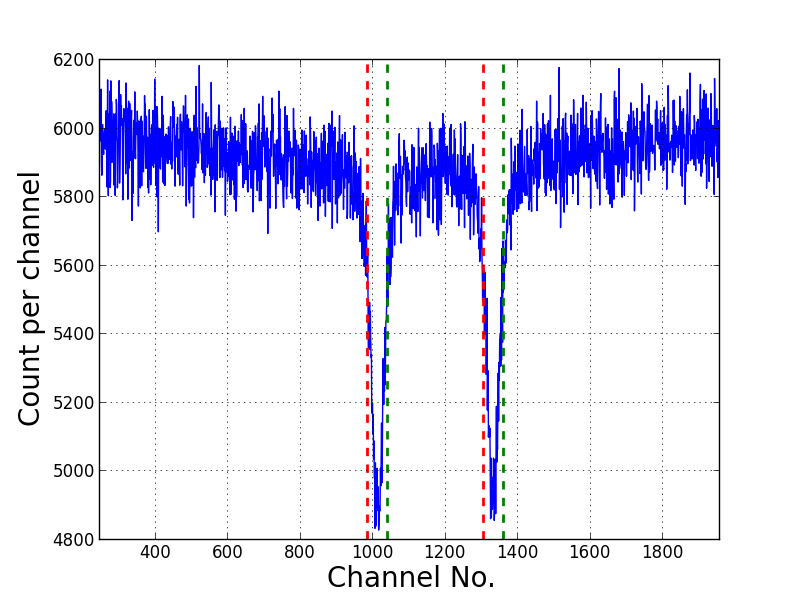
\includegraphics[width=6cm]{../FeSO4_Fe2SO4_3/02-19-FeSO4_raw.png}\\
        \begin{block}{Isomer shift ($\varepsilon$) and quaduapole splitting ($\delta$).}
          \begin{tabular}{|c|c|}
            \hline
            $\varepsilon$&$5.9(1.4)\cdot10^{-8}eV$\\\hline
            $\delta$&$1.562(2)\cdot10^{-7}eV$\\\hline
          \end{tabular}
        \end{block}
      \end{center}
    }
  \end{columns}
\end{frame}

\def\timeleft{2:00->0:30}
\begin{frame}{Temperature effect.}
  \begin{columns}
    \column{6cm}
    \begin{block}{Samples}
      \begin{itemize}[<+->]
      \item Classic:
        \[E_k=\frac{3}{2}k_BT\]
      \item Debye $T^3$ approximation:
        \[E_k=\frac{3\pi^4*k_B*T^4}{10\Theta_D^3}\]
      \item Exact Debye Model:
        \[E_k=\frac{9k_BT^4}{10\Theta_D^3}D_3\left(\frac{T}{\Theta_D}\right)\]
      \end{itemize}
    \end{block}
    \column{6cm}
    \visible<+->{
      \begin{center}
        \begin{tabular}{|c|c|}
          \hline
          $t_{low}$&$21(1)^{\circ}C$\\\hline
          $t_{high}$&$130(5)^{\circ}C$\\\hline
          $\delta/E$&$1.86(69)\cdot 10^{-13}$\\\hline
        \end{tabular}\vspace{.5cm}
        \begin{tabular}{|c|c|}
          \hline
          Model&$E_k$\\\hline
          Classic&$1.409(12)\cdot 10^{-2}eV$\\\hline
          Debye $T^3$&$4.59(22)\cdot 10^{-1}eV$\\\hline
          Exact Debye&$1.304(84)\cdot 10^{-2}eV$\\\hline
          (Measured)&$0.99(36)\cdot 10^{-2}eV$\\\hline
        \end{tabular}
      \end{center}
    }
  \end{columns}
\end{frame}

\def\timeleft{0:30->0:00}
\section{Conclusion.}
\begin{frame}{Conclusion.}
  \begin{block}{}
    \begin{itemize}[<+->]
    \item
      Calibrated the velocity using laser.
    \item
      Measured M�ssbauer spectrum of a variety of materials.
    \item
      Calculated different kinds of splitting and shifting.
    \end{itemize}
  \end{block}
\end{frame}

\begin{frame}{}
\end{frame}

\begin{frame}{}
  \begin{columns}
    \column{5cm}
    \begin{block}{Effects}
      \begin{itemize}
      \item
        Isomer Shift:
        \[\varepsilon\]
      \item
        Zeeman effect:
        \[g_0,\ g_1\]
      \item
        Quadrapole Splitting:
        \[\delta\]
      \end{itemize}
    \end{block}
    \column{6.5cm}
    \begin{align}
      \Delta E_1=&\varepsilon-\frac{g_0}2-\frac{3g_1}{2}-\frac{\delta}{2}\\
      \Delta E_2=&\varepsilon-\frac{g_0}2-\frac{g_1}{2}+\frac{\delta}{2}\\
      \Delta E_3=&\varepsilon-\frac{g_0}2+\frac{g_1}{2}+\frac{\delta}{2}\\
      \Delta E_4=&\varepsilon+\frac{g_0}2-\frac{g_1}{2}+\frac{\delta}{2}\\
      \Delta E_5=&\varepsilon+\frac{g_0}2+\frac{g_1}{2}+\frac{\delta}{2}\\
      \Delta E_6=&\varepsilon+\frac{g_0}2+\frac{3g_1}{2}-\frac{\delta}{2}
    \end{align}
  \end{columns}
\end{frame}

\begin{frame}{}
  \includegraphics[width=7cm]{../all_data/02-28-FeC2O4_diff.png}
\end{frame}

\end{document}
